The following results are based on simulations of the model with parameter values given in
\autoref{tab:parameter}.  The grid size was 101 patches by 101 patches.

\begin{table}
  \begin{tabular}{|l|l|l|l|}
    \hline
    % after \\: \hline or \cline{col1-col2} \cline{col3-col4} ...
    Parameter Description & Symbol & Value &  \\ \hline  \label{parameter}
    Total number of animals & b & 1,000 & fixed  \\ \hline
    Maximum time & $t_{max}$ & 1,200 seconds & fixed \\ \hline
    Fraction of blooms at one time & a & 0.2 & fixed \\ \hline
    Maximum fraction of available flowers & $\eta$ & 0.75 & fixed \\ \hline
    Search radius & r & 1.0 & fixed \\ \hline
    Number of flowers per plant & $\phi$ & 100 & fixed \\ \hline
    Probability of pollination   & $\rho$ & 0.4286 & calculated \\ \hline
    Number of plants & n & 1000 & fixed \\ \hline
    Time spent at each plant & $t_{plant}$ & 100 seconds & fixed \\ \hline
  \end{tabular}
  \caption{Parameter Values}
  \label{tab:parameter}
\end{table}

The standard error was calculated by dividing the sample standard deviation by the square root of
the total number of samples.   The standard errors were all less than 1\% on average, so will not be
shown due to the small size.

Determining the distance animals travel during a foraging trip is important factor for their
survivability.  In order for an animal to survive it must find enough food foraging without losing
too much energy.  In this study the density of plants is varied, which can directly affect the
amount of foraging the animals will be able to achieve in a set amount of time.  The higher the
density the greater the potential for the animal to forage.  The maximum angle is also varied.  The
relationship of this angle with respect to foraging is a more complicated one.  In terms of
foraging, a very small maximum turning angle may not result in successful foraging due to the paths
are too linear.  On the other hand, a maximum turning angle which is too large can result in
searching patterns that repetitively cover the same area over and over again.

%{\emph{Average Path Distance}}
\begin{figure}
  \begin{center}
  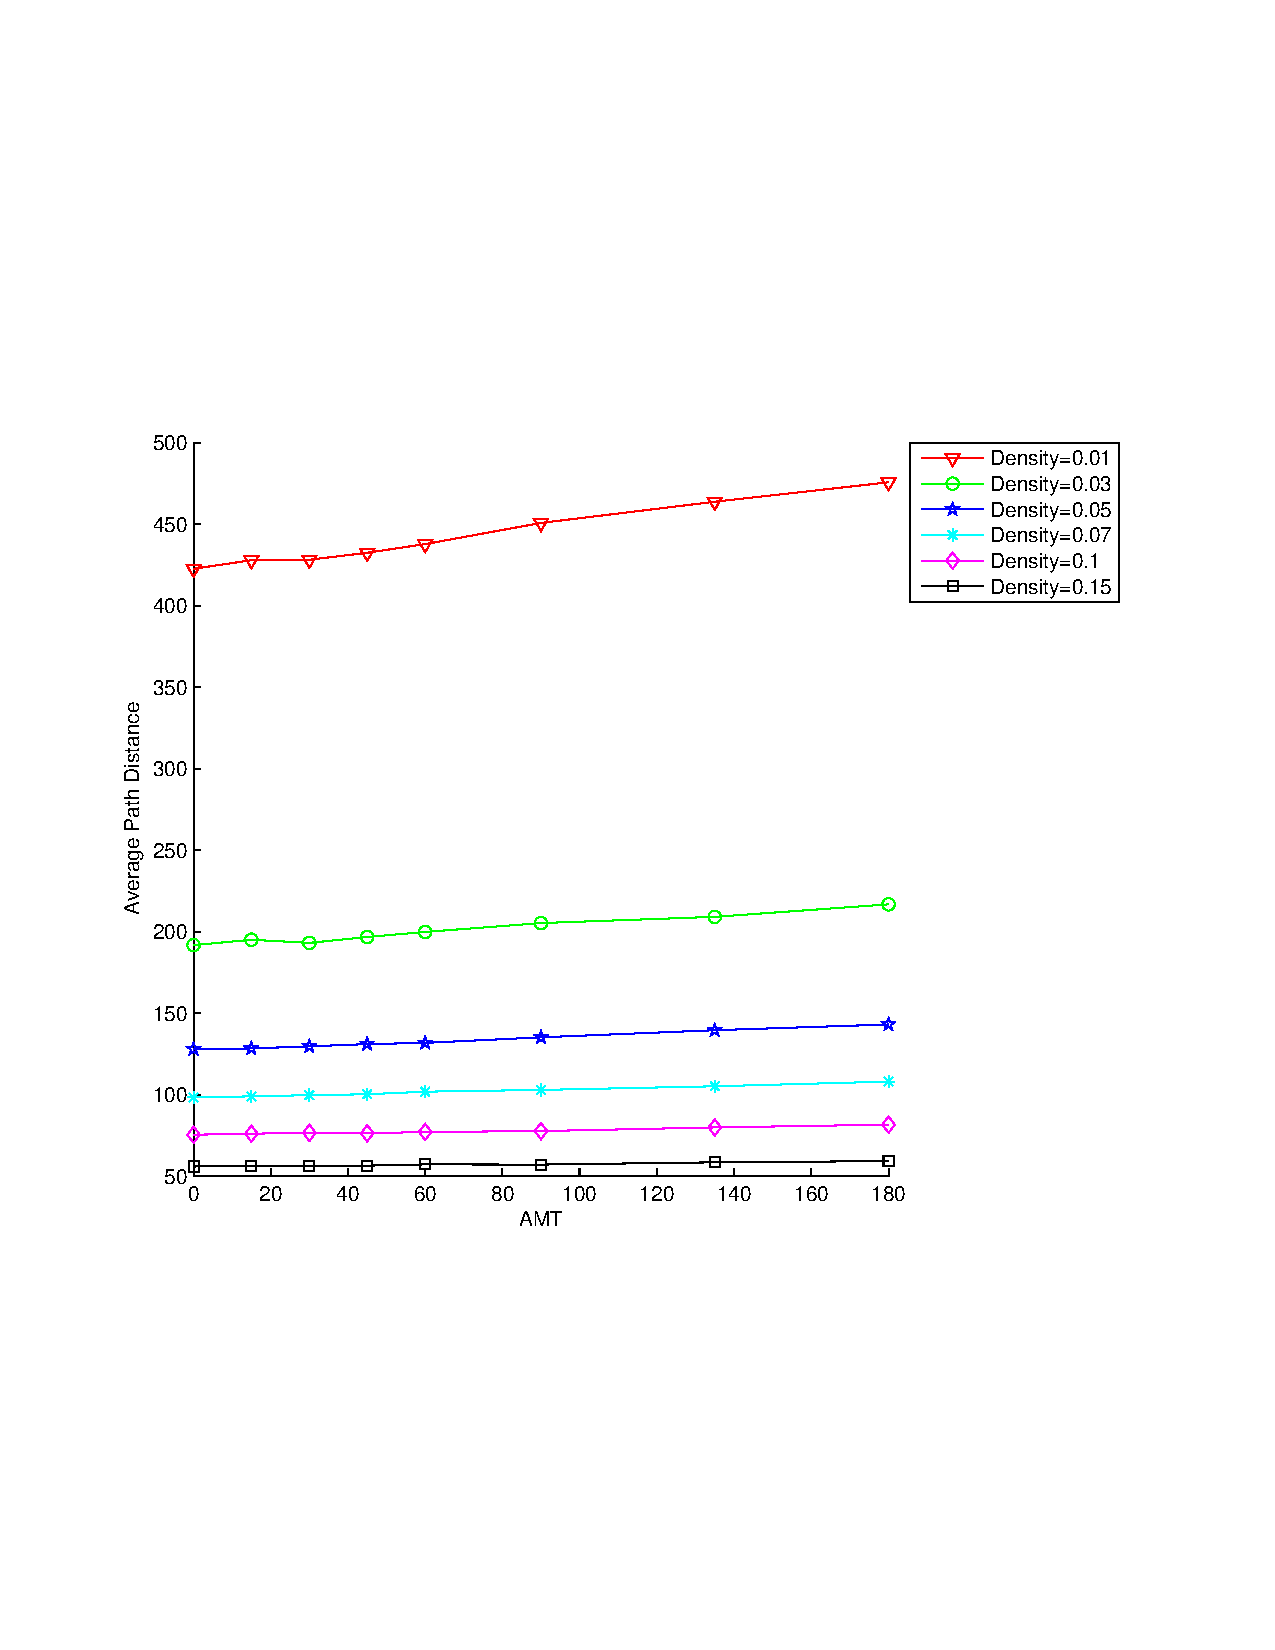
\includegraphics[scale=0.5, trim=0 240 50 300]{PathVsAMT.pdf}
  \end{center}
  \caption{\small Average Path Distance vs. Turning Angle for Various Plant Densities}
  \label{AvgPathN}
\end{figure}

In \autoref{AvgPathN} the average distance traveled for each animal decreases with increasing
density due to higher foraging success.  In this situation the animals will spend more time on
plants since they can find plants more readily.  The maximum turning angle does not have a large
effect on on the distance.  There is a modest effect of maximum turning angle on low plant density
where the larger the angle increases the average distance due to less success of foraging.

The average maximum distance traveled by animals, see \autoref{AvgMaxDBees}, is affected by both
the turning angle and plant density. As with the average path distance, the maximum distance
decreases with higher density which decreases the overall travel time for the animals.  Though in
this case due to the movement patterns the angle has a large effect on maximum distance especially
at lower densities.  As the maximum angle decreases the animals are more likely to travel directly
away from their starting points increasing the maximum distance traveled.

%\subsubsection*{\emph{Average Maximum Distance}}
\begin{figure}
  \begin{center}
  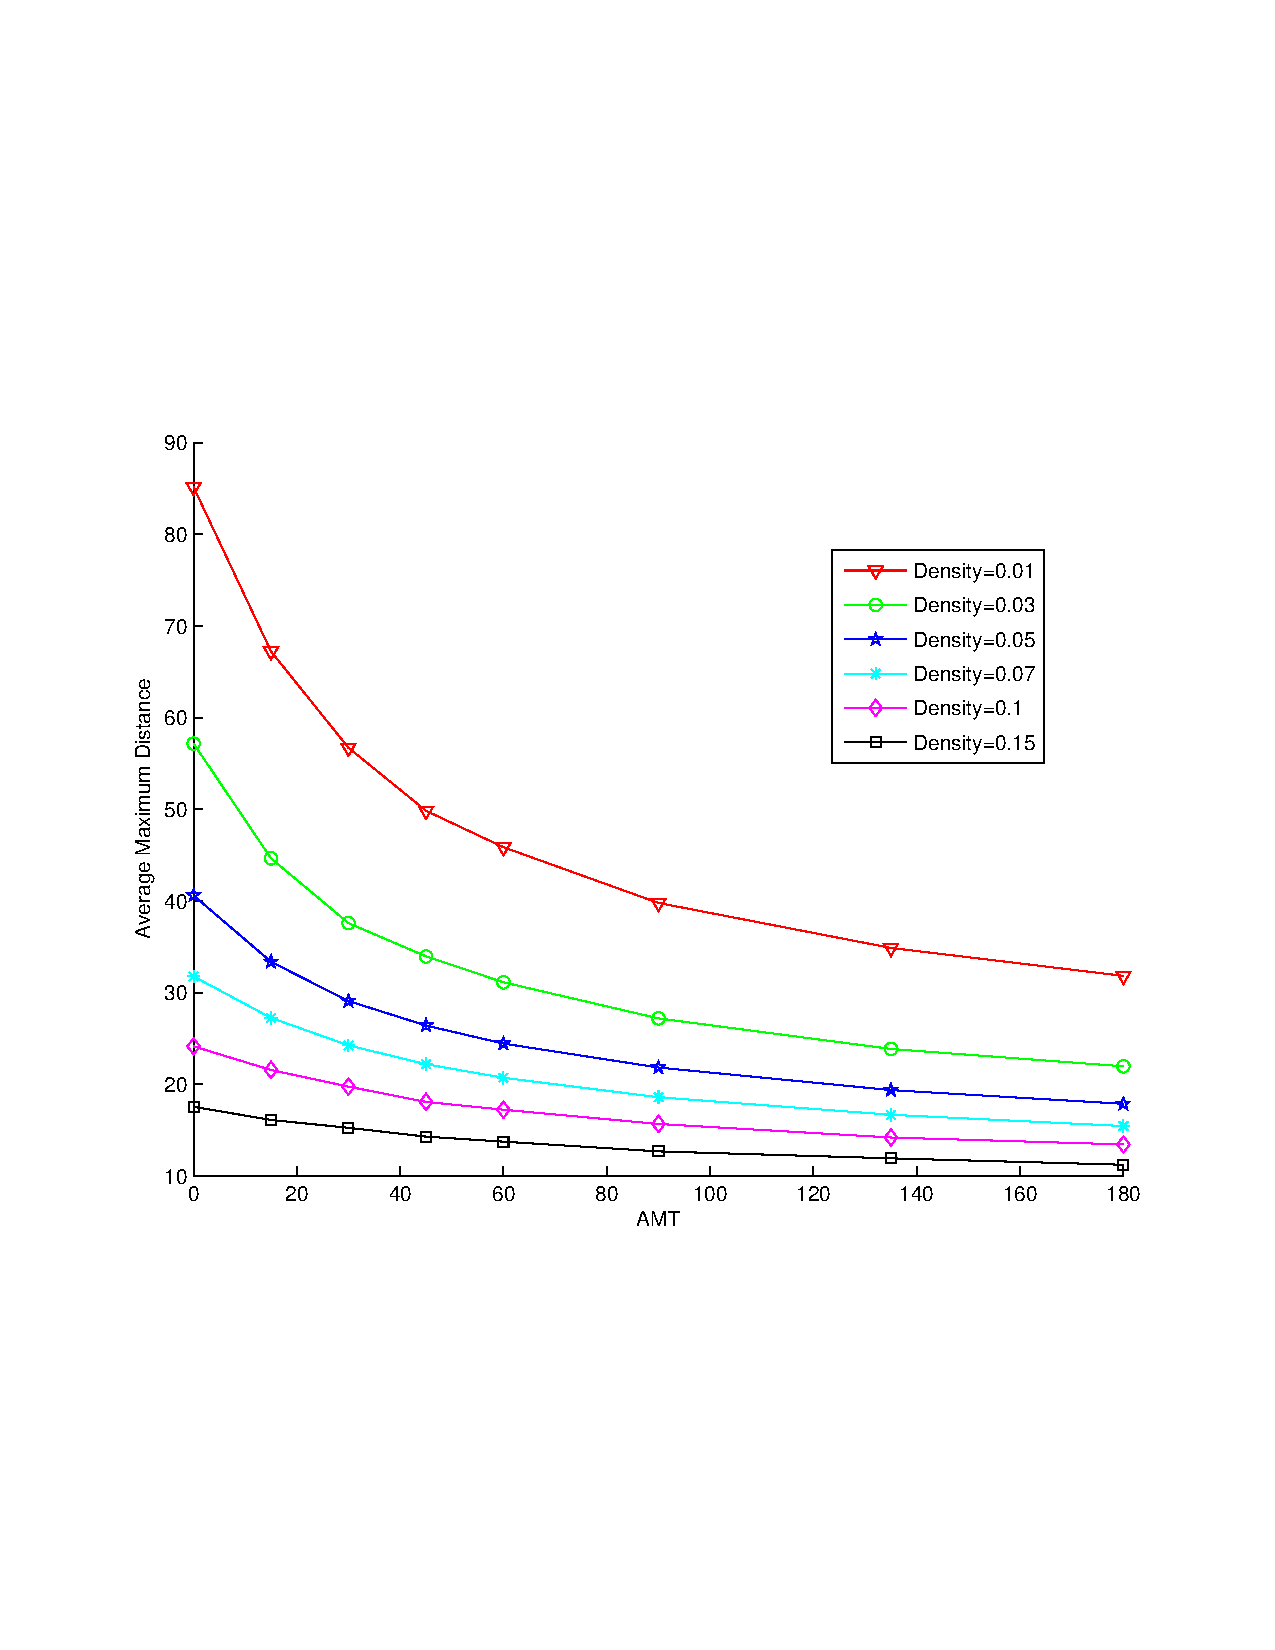
\includegraphics[scale=0.5, trim=50 240 50 300]{MaxDVsAMT.pdf}
  \end{center}
  \caption{\small Average Maximum Distance vs. Turning Angle for Various Plant Densities}
  \label{AvgMaxDBees}
\end{figure}

For a plant density of 0.01 and AMT = $0^\circ$ the average maximum distance is quadruple of the
average maximum distance for a plant density of 0.01 and AMT = $180^\circ$. For a higher plant
density of 0.15 the average maximum distance is 50\% larger. Thus, a purely random diffusion process
results in shorter average maximum distances as compared to smaller turning angles, and as was seen
with the average pollination distance the effect of turning angle is more pronounced for smaller
plant densities. Again, this is expected since for higher plant densities the animal direction is
reset more often and therefore the animal path becomes more and more like a purely random walk.

%\subsubsection*{\emph{Average Pollination Distance}}
\begin{figure}
  \begin{center}
  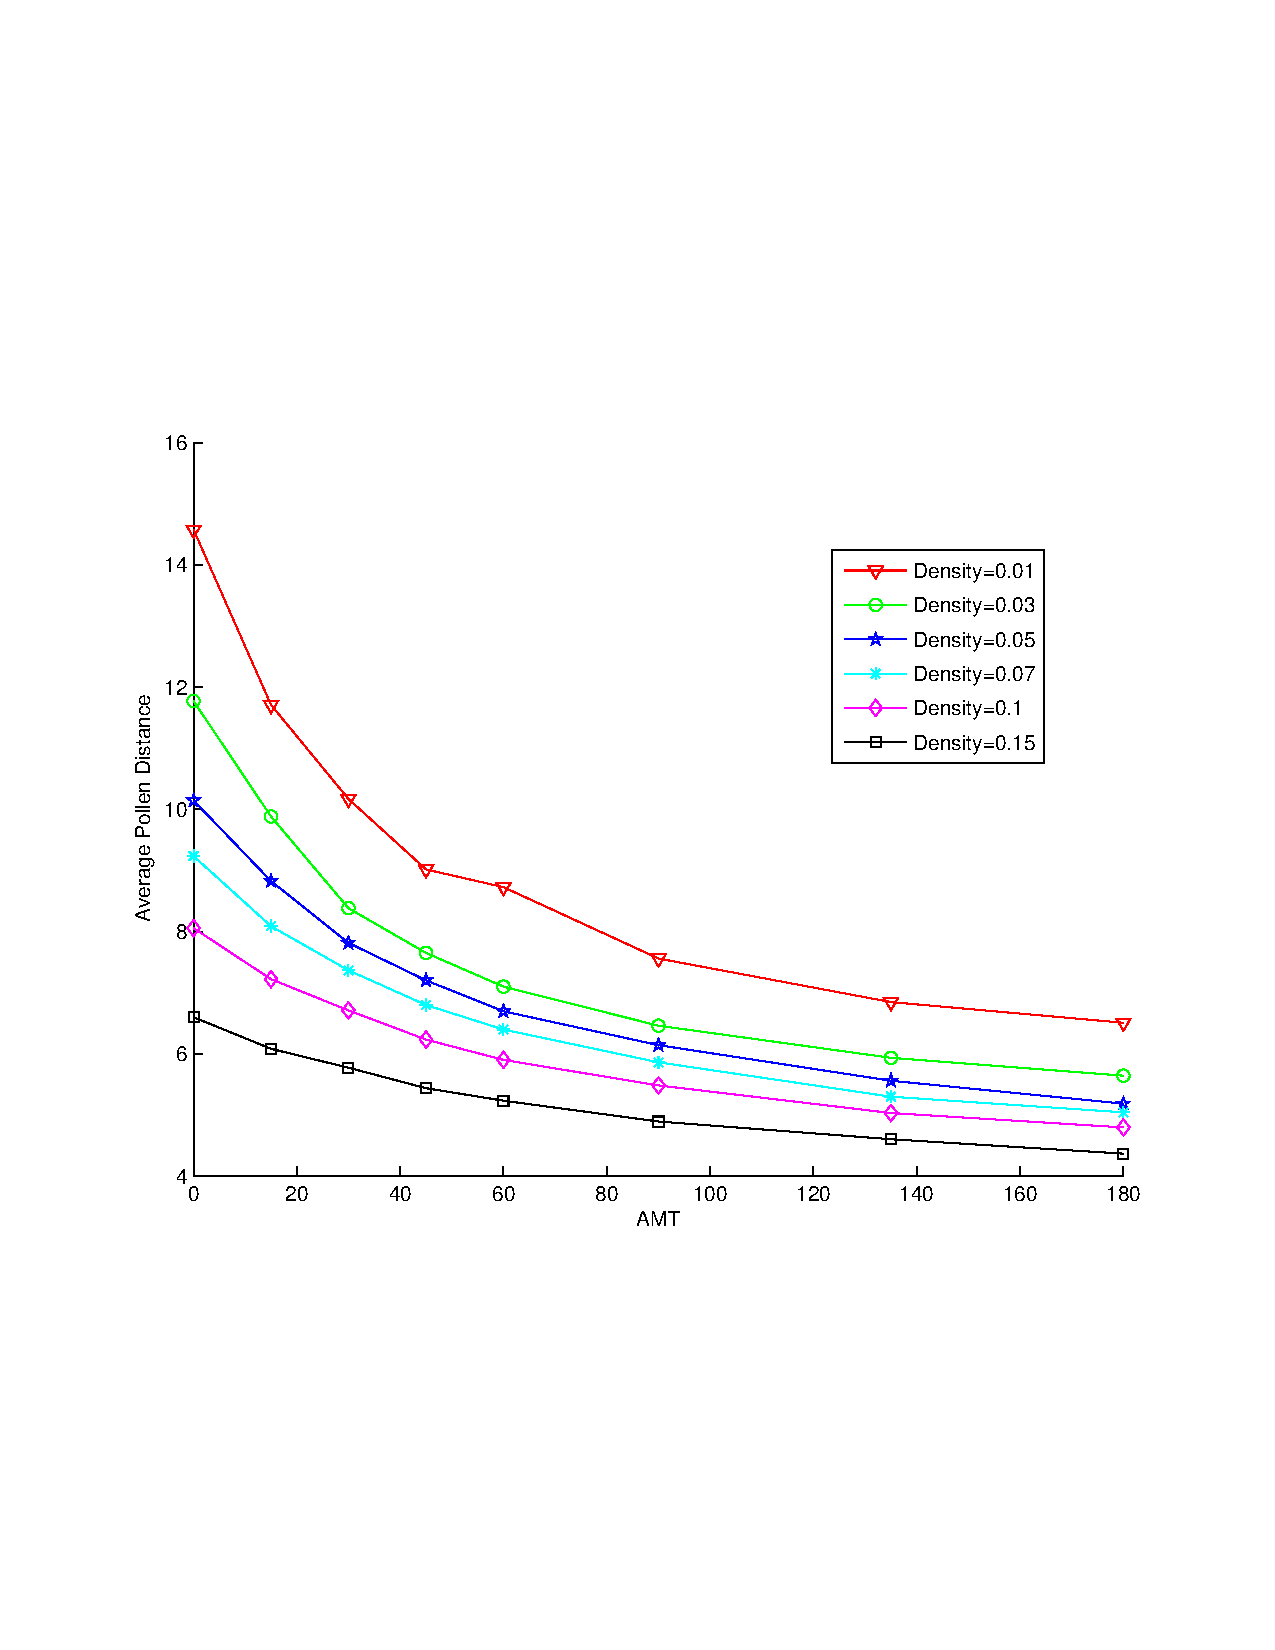
\includegraphics[scale=0.5, trim=50 240 50 300]{PollenDVsAMT.pdf}
  \end{center}
  \caption{\small Average Pollination Distance vs. Turning Angle for Various Plant Densities}
  \label{AvgDist}
\end{figure}

The average pollination distance, see \autoref{AvgDist}, decreases with increasing density due to
the greater likelihood of pollinating nearby trees.  As with the average maximum distance, as the
maximum angle decreases the animal is likely to travel farther from its initial position which
allows for longer pollination distances.

For a plant density of 0.01 and AMT = $0^\circ$ the average maximum pollination distance is
approximately triple of that for the same plant density and AMT = $0^\circ$. Additionally, for plant
density of 0.15 and AMT = $0^\circ$ the average pollination distance is approximately double of the
average pollination distance for the same density and AMT = $180^\circ$. Clearly, the average
pollination distance for wind dispersal is less than that of an average pollination distance for an
animal that follows a straighter path for any of the simulated plant densities.

%\subsubsection*{\emph{Average Maximum Pollination Distance}}
\begin{figure}
  \begin{center}
  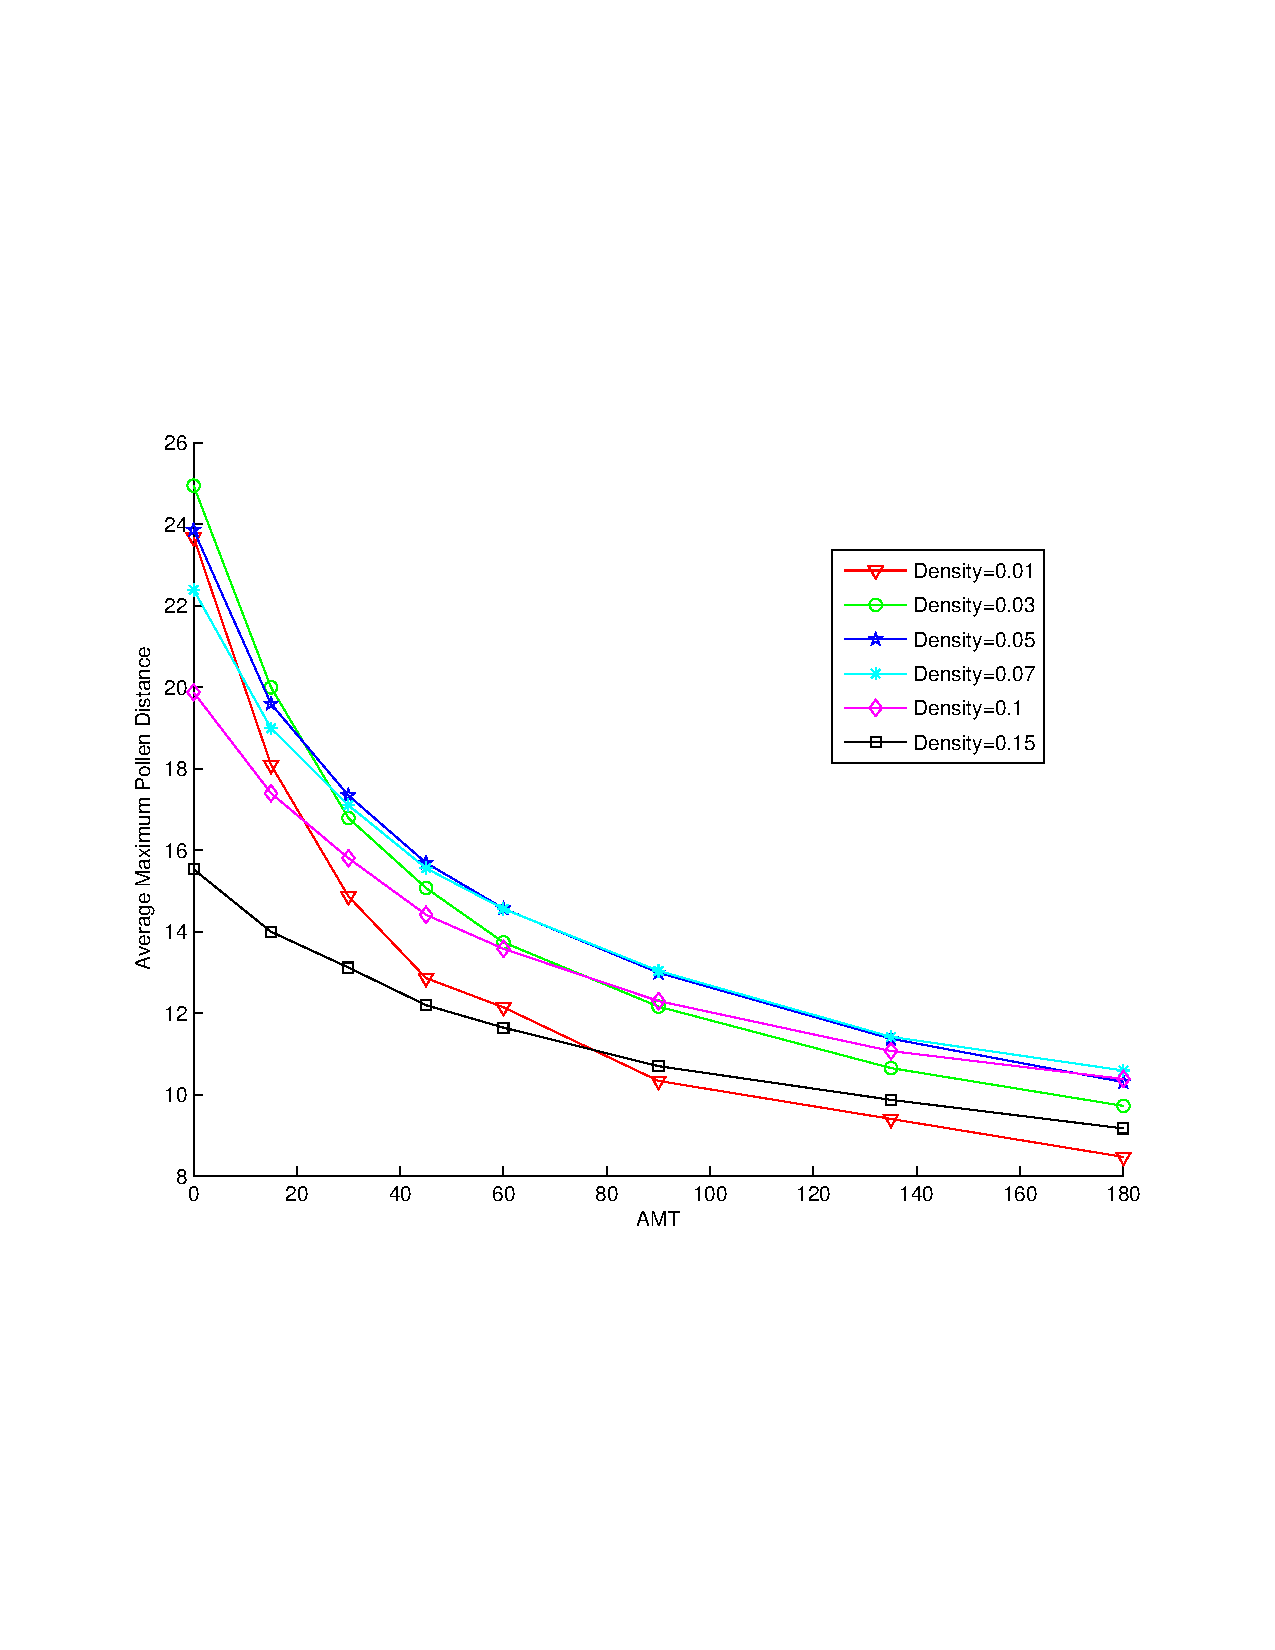
\includegraphics[scale=0.5, trim=50 240 50 300]{MaxPollenVsAMT.pdf}
  \end{center}
  \caption{\small Average Maximum Pollination Distance vs. Turning Angle for Various Plant Densities}
  \label{AvgMaxDTreesN}
\end{figure}

The average maximum pollination distance has a much more complicated relationship with density and
maximum turning angle, see \autoref{AvgMaxDTreesN}.  The average maximum pollination distance
decreases as maximum turning angle increases from $0^{\circ}$ to $180^{\circ}$ across all densities.
This is due to animals covering a shorter distance for higher turning angles, and therefore the
plants that are visited will be closer together on average. 

Additionally, we see that the resultant average maximum pollination distance for a purely random
diffusion process is marketably lower than those for correlated random walks resulting in straighter
animal paths. Thus, wind dispersal will result in an average maximum pollination distance that is
less than the average maximum pollination distance for a correlated random walk. Thus, one might
expect that wind dispersal of pollen results in a smaller areal extent of gene flow as compared to
animal mediated gene flow.

The density affects the maximum pollination distance in a more complex fashion.  The higher the
density the more gradual the decrease is in the maximum pollination distance as the maximum turning
angle increases.  Whereas for lower densities this decrease is much larger.  This is likely due to
the fact that at lower densities pollination occurs less frequently with a larger variability of
maximum pollination distances.

%\subsubsection*{\emph{Average Weighted Diversity of Fathers}}
\begin{figure}
  \begin{center}
  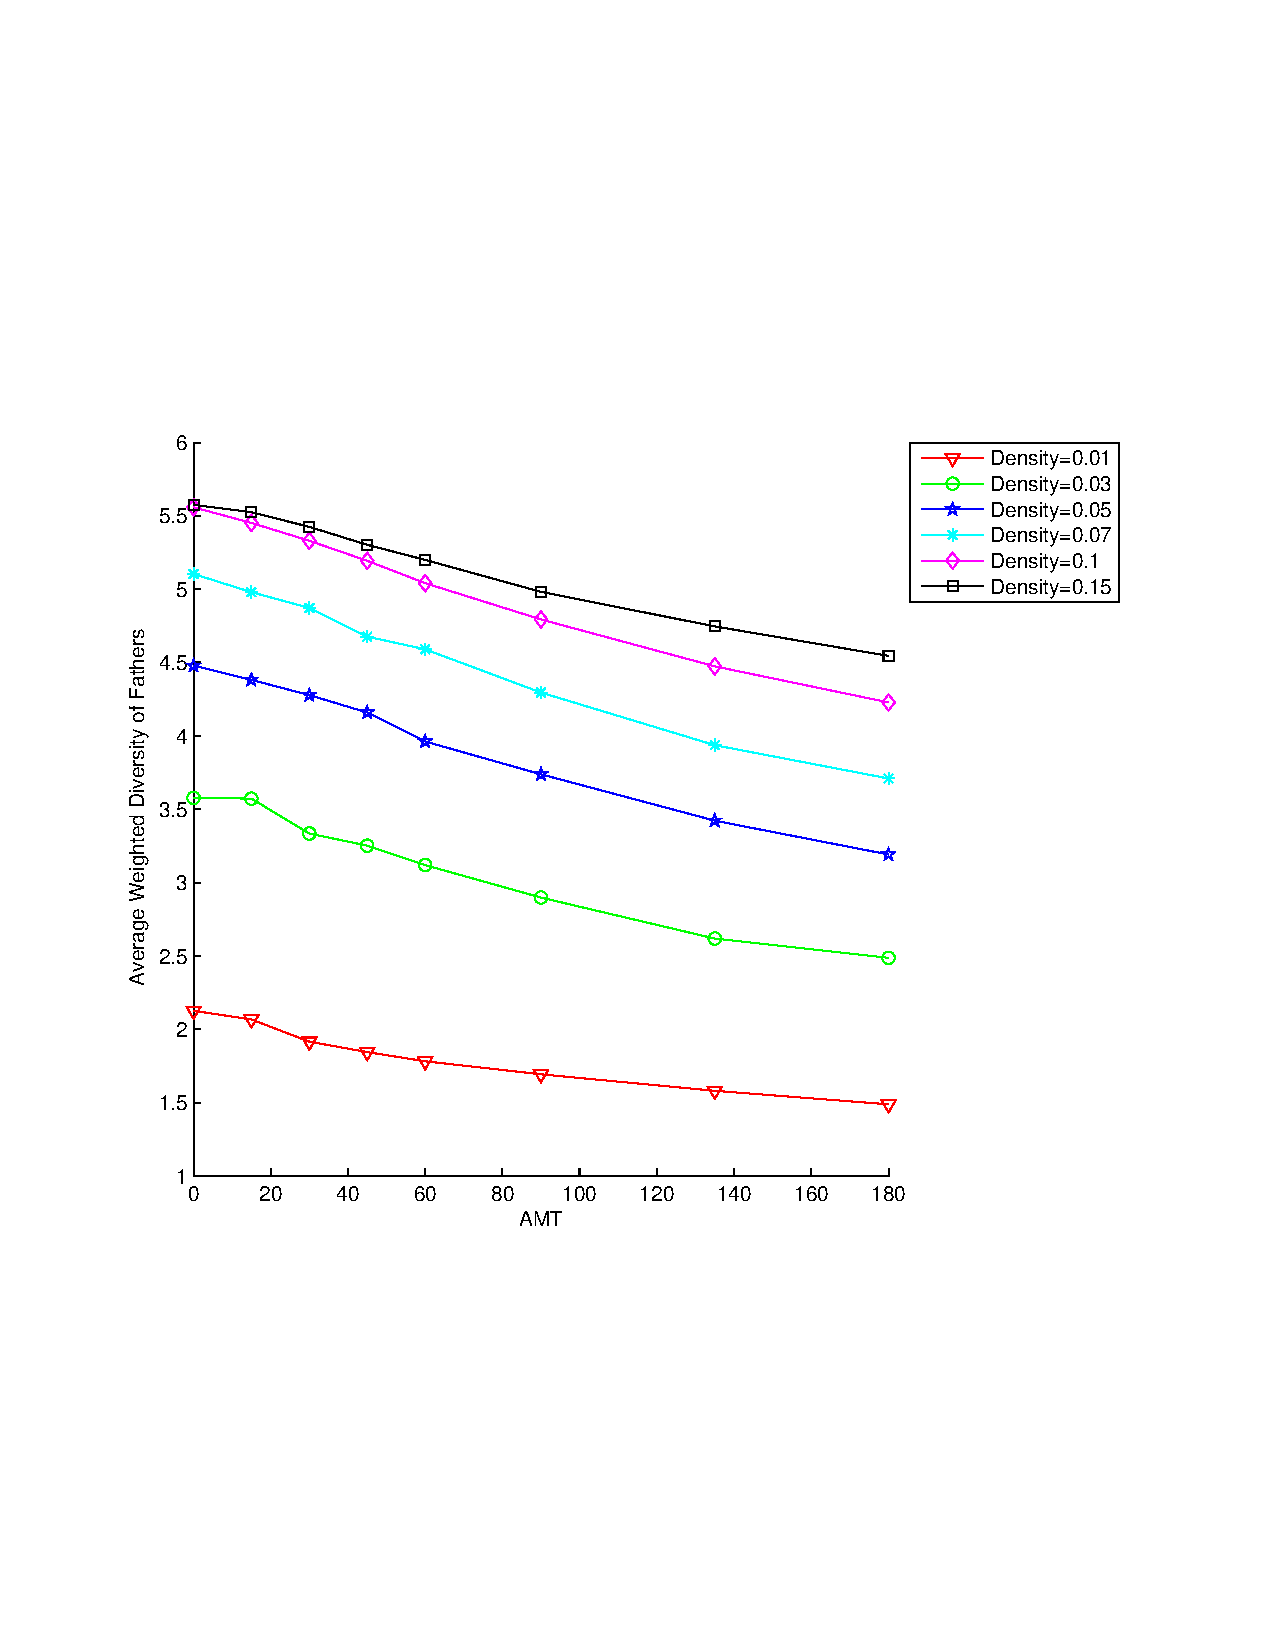
\includegraphics[scale=0.5, trim=0 240 50 300]{WDFvsAMT.pdf}
%  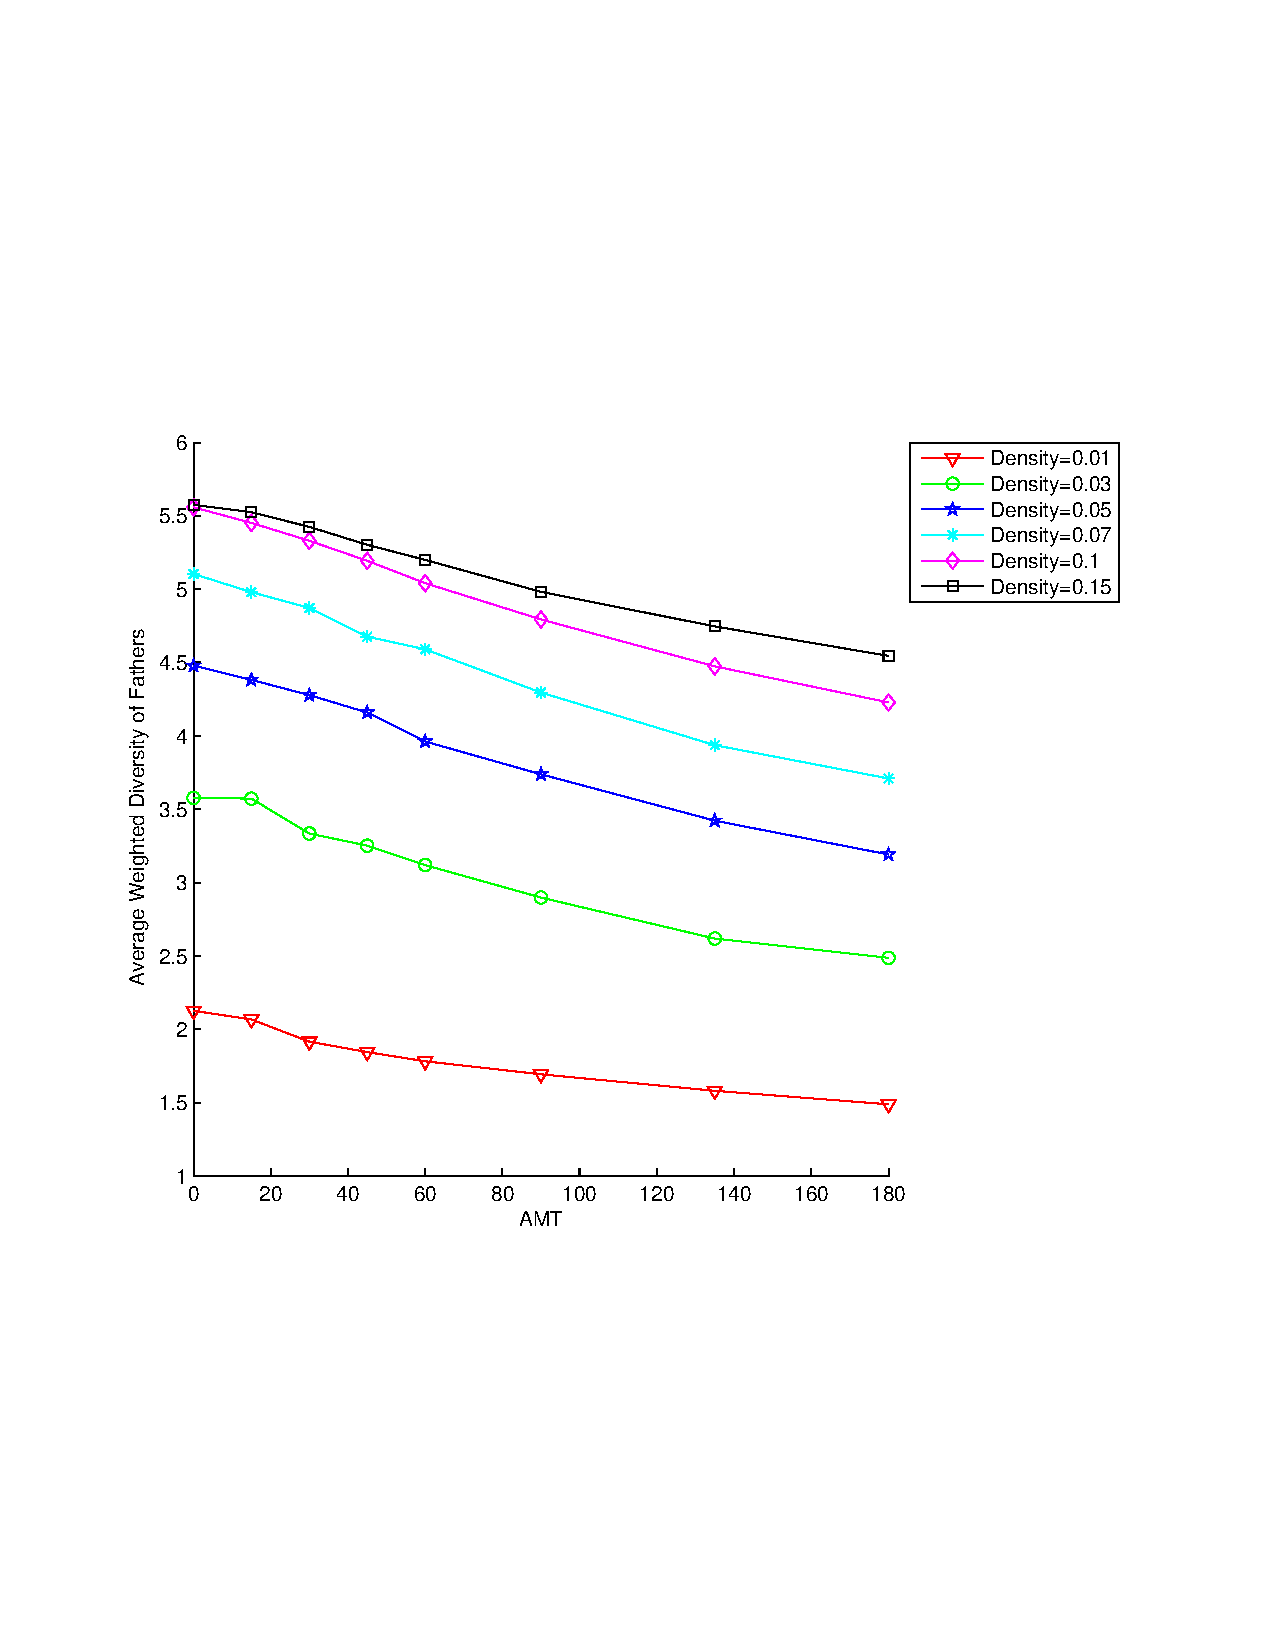
\includegraphics[width=1.0\textwidth,height=0.5\textheight]{WDFvsAMT.pdf}
  \end{center}
  \caption{\small Average Weighted Diversity of Fathers vs. Turning Angle for Various Plant Densities}
  \label{EFathers}
\end{figure}

In general there is a small decrease in the average weighted diversity of fathers as the maximum
turning angle increases, see \autoref{EFathers}. With higher maximum turning angles the search
patterns tend to be more circular lowering the overall diversity that a plant will see.  On the
other hand, by increasing the density, plants will see an increase in diversity due to the larger
amount of plants near by.  This increase is lessens at higher densities due to the limited foraging
time of the pollinators.
